\underbar{\textbf{\large Ejercicio 2:}} Dado el siguiente programa:
\begin{center}
  \begin{lstlisting}[frame = single]
struct B {
  void f ( ) { std::cout << "f ( ) de B" << std::endl; }
  };

struct D:B {
  void f ( ) { std::cout<<"f ( ) de D" << std::endl;}
  };

void f(B b) {
  std::cout << "f ( ) externa"<< std::endl;
  b.f( );
  }

int main(){
  B b;
  D d;
  f(b);
  f(d);
}
  \end{lstlisting}
\end{center}

\begin{enumerate}[label = \alph*)]
  \item Diga si tiene error de compilación o ejecución. Modifique el código para solucionarlo y después escribe lo que imprime. Si no, sólo lo que imprime.
  
  No hay ningún error en el código por tanto, ejecuta correctamente:
  \begin{verbatim}
    f() externa
    f() de B
    f() externa
    f() de B
  \end{verbatim}
  Imprime esto debido a que aunque el método void f(B b) reciba un objeto de tipo D, se llama al método B::f() ya que B no es una clase polimórfica y se tiene en cuenta el tipo del objeto que se recibe (de tipo B).
  \item Repite el anterior pero suponiendo \textbf{B::f()} como virtual.
  
  Da como resultado lo mismo.

  \item Repite el anterior pero teniendo en cuenta que el parámetro función externa \texttt{f()} se recibe por referencia.
  
  Si mantenemos como virtual B::f() y modificamos el método void f() haciendo que reciba una referencia, vemos que ahora imprime:

  \begin{verbatim}
    f() externa
    f() de B
    f() externa
    f() de D
  \end{verbatim}
  Ahora vemos que llama al método D::f(), esto es debido a que ya no le pasamos un objeto, si no una referencia a dicho objeto, y esto sumado a que B es una clase polimorfica hace que el compilador sepa que tiene que llamar al método D::f().
  \item Repita el 2º apartado suponiendo que la definición de f()(externa) se ha cambiado a: \texttt{void f(B *b) {std::count<< "f() externa"<<std::endl;
  b.f(); }}

  Ahora el método void f() recibe una dirección de memoria , por tanto, primero de todo necesitamos hacer cambios en el main, ya que le tenemos que pasar una referencia al método:
  \begin{minted}[breaklines]{C++}
struct B {
  virtual void f () { std::cout << "f ( ) de B" << std::endl; }
};
struct D:B {
  void f () { std::cout<<"f ( ) de D" << std::endl;}
};

void f (B* b) {
  std::cout << "f ( ) externa"<< std::endl;
  b->f(); //cambiamos b.f() por b->f();
}

int main(){
  B b;
  D d;
  f(&b); //ahora le pasamos direcciones de memoria
  f(&d);
}
  \end{minted}
  Tanto una referencia como un puntero están involucrados en la manipulación de direcciones de memoria en C++. El resultado después de aplicar los cambios es el mismo que en el apartado anterior.

  En la explicación previa, utilizamos una referencia a un objeto pasado por valor mediante void f(B\& b). Si ese objeto es de tipo D, se llamará a D::f(). Ahora, al utilizar f(B* b), estamos manipulando un objeto apuntado por un puntero. Si este puntero apunta a un objeto de tipo D, se llamará a D::f(), siempre y cuando la clase B sea polimórfica, es decir, tenga al menos una función virtual.
\end{enumerate}

\newpage
\underbar{\textbf{\large Ejercicio 3:}} Para una aplicación de geometría se dispone de la clase Punto y es necesario desarrollar las clases Cuadrilátero, Trapezoide, Paralelogramo, Rombo, Rectángulo Y Cuadrado. Los atributos de estos polígonos serán los cuatro puntos que los forman en orden consecutivo.
\begin{enumerate}[label = \alph*)]
  \item Dibuje el diagrama de clases atendiendo a las siguientes definiciones:
  \begin{itemize}
    \item Cuadrilátero: polígono de cuatro lados.
    \item Trapezoide: cuadrilátero con ningún lado paralelo a otro.
    \item Trapecio: cuadrilátero con sólo dos lados paralelos.
    \item Paralelogramo: cuadrilátero con sus lados paralelos dos a dos.
    \item Rombo: paralelogramo con los cuatro lados iguales.
    \item Rectángulo: paralelogramos cuyos lados forman ángulos rectos entre sí.
    \item Cuadrado: paralelogramo cuyos lados son iguales y forman ángulos rectos entre sí.
  \end{itemize}

  Como cualquier figura contiene 4 puntos y todas estas figuras se pueden obtener de una en común (a partir de un cuadrilátero, podemos obtener Trapezoide, Trapecio y Paralelogramo) y a través de un Paralelogramo obtenemos (Rombo, Rectángulo y Cuadrado), por tanto, podemos implementarlo de la siguiente manera:
  \begin{center}
    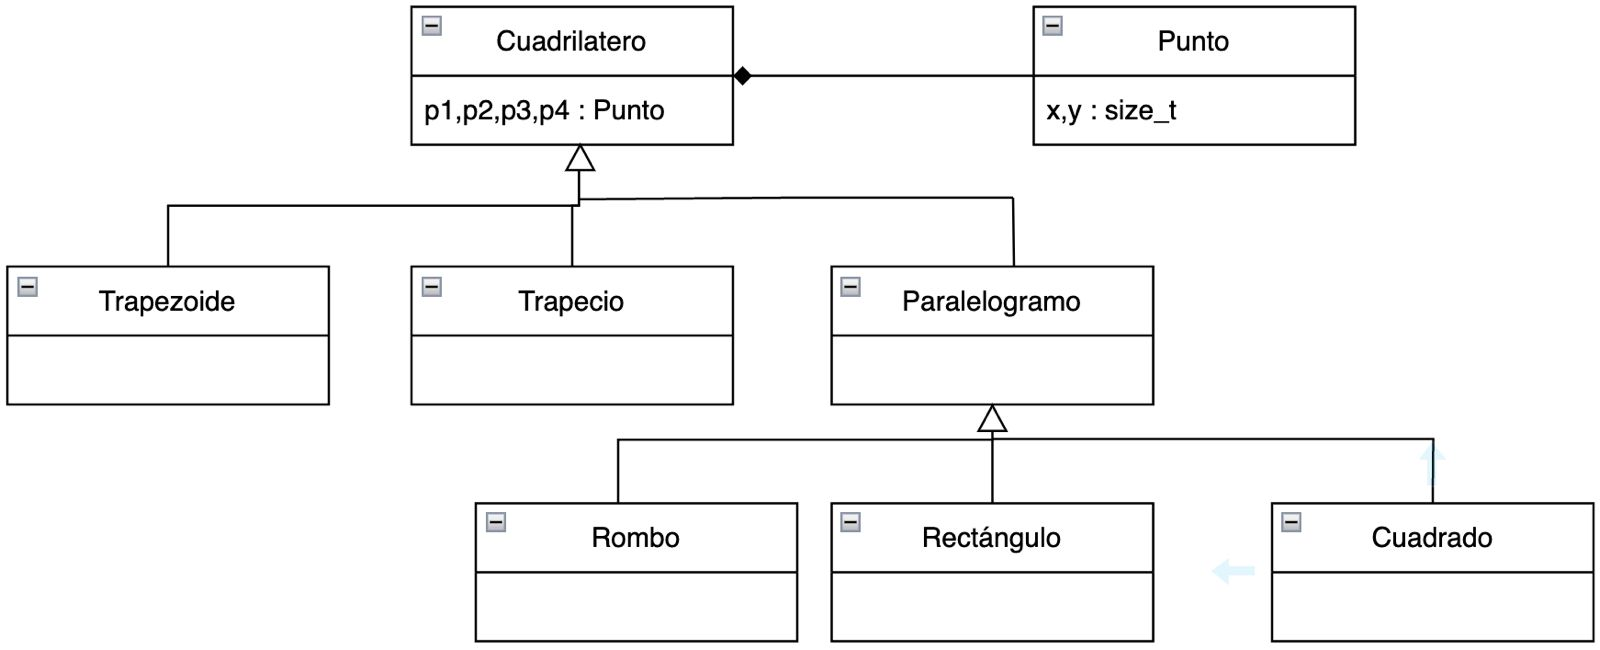
\includegraphics[width=0.9\textwidth]{assets/WhatsApp Image 2024-06-14 at 20.28.31.jpeg}
  \end{center}
  \item Declare (solo la interfaz) todas las clases considerando que se requieren, entre otros, métodos para calcular el perímetro y para imprimirlos (el procedimiento de impresión será diferente para todos y cada uno de los polígonos).
  
  \begin{minted}[breaklines]{C++}
class Punto{
  public:
    Punto(size_t a, size_t b):x_(a),y_(b){}
    inline size_t x()const {return x_;}
    inline size_t y()const {return y_;}
  private:
    size_t x_,y_;
};

class Cuadrilatero{
  public:
    Cuadrilatero(Punto p1,Punto p2, Punto p3, Punto p4):
      p1_(p1),p2_(p2),p3_(p3),p4_(p4){}
      double perimetro()const{
        return longitud(p1_,p2_)+longitud(p2_,p3_)+longitud(p3_,p4_)+longitud(p4_,p1_);
      }
    virtual void impresion () const = 0;
  protected: //Lo hacemos protected, para que puedan tener acceso las clases derivadas
    Punto p1_,p2_,p3_,p4_;
    double longitud(const Punto& p1, const Punto& p2) const {
    return sqrt(pow(p1_.x() - p2_.x(), 2) + pow(p1_.y() - p2_.y(), 2));
    }
};

class Trapezoide : public Cuadrilatero{
  public:
    Trapezoide(Punto& p1,Punto& p2,Punto& p3,Punto& p4):Cuadrilatero(p1,p2,p3,p4){}
    //Método específico llamado impresion
    virtual void impresion()const override{
      std::cout<<"El perimetro del Trapezoide es: "<<Cuadrilatero::perimetro()<<std::endl;
    }
};
class Trapecio : public Cuadrilatero{
  public:
    Trapecio(Punto& p1,Punto& p2,Punto& p3,Punto& p4):Cuadrilatero(p1,p2,p3,p4){}
    //Método específico llamado impresion
    virtual void impresion()const override{
      std::cout<<"El perimetro del Trapecio es: "<<Cuadrilatero::perimetro()<<std::endl;
    }
};
class Paralelogramo: public Cuadrilatero{
  public:
    Paralelogramo(Punto& p1,Punto& p2,Punto& p3,Punto& p4):Cuadrilatero(p1,p2,p3,p4){}
    //Método específico llamado impresion
    virtual void impresion()const override{
      std::cout<<"El perimetro del Paralelogramo es: "<<Cuadrilatero::perimetro()<<std::endl;
    }
};
class Rombo : public Paralelogramo{
  public:
    Rombo(Punto& p1,Punto& p2,Punto& p3,Punto& p4):Paralelogramo(p1,p2,p3,p4){}
   virtual void impresion()const override{
      std::cout<<"El perimetro del Rombo es: "<<Cuadrilatero::perimetro()<<std::endl;
    }
};
class Rectangulo : public Paralelogramo{
  public:
    Rectangulo(Punto& p1,Punto& p2,Punto& p3,Punto& p4):Paralelogramo(p1,p2,p3,p4){}
   virtual void impresion()const override{
      std::cout<<"El perimetro del Rectangulo es: "<<Cuadrilatero::perimetro()<<std::endl;
    }
};
class Cuadrado : public Paralelogramo{
  public:
    Cuadrado(Punto& p1,Punto& p2,Punto& p3,Punto& p4):Paralelogramo(p1,p2,p3,p4){}
   virtual void impresion()const override{
      std::cout<<"El perimetro del Cuadrado es: "<<Cuadrilatero::perimetro()<<std::endl;
    }
};
  \end{minted}
\end{enumerate}